\documentclass[conference]{assets/latex/IEEEtran}
\usepackage{amsmath}
\usepackage{graphicx}
\graphicspath{{assets/latex/}}

\begin{document}

\title{CS6524 Lab 4: Optical Flow and Kalman Tracking Through Occlusion}
\author{\IEEEauthorblockN{Naem Haq, Patrick Walsh, and James Doherty}
\IEEEauthorblockA{Immersive Software Engineering, University of Limerick\\
Group 04}}
\maketitle

\begin{abstract}
We tracked a moving target through occlusion by combining sparse
Lucas--Kanade optical flow with a foreground silhouette and a Kalman filter.
The tracker reacquired the target in all three supplied clips and the bonus
clip. At reacquisition, the distance between the uncorrected prediction and
the new position measurement ranged from 70.8 to 154.0 source pixels.
These discrepancies show why a separate prediction-only trajectory is
useful when assessing the motion model.
\end{abstract}

\section{Method}

\subsection{Target detection and optical flow}
We processed frames at 640 pixels wide, preserving the original aspect
ratio. To locate the target, we subtracted a fixed background frame from
the current colour frame, intersected the resulting change mask with a
clip-specific HSV range, and excluded the occluder and areas outside the
expected motion band. After morphological closing and opening, the detector
ranked connected components by log area and, once tracking began,
penalised distance from the predicted position. That penalty weakened as
the gap grew so a displaced target could be reacquired.

The tracked point was the foreground centroid. In clip 02, we used the
centre of the pen's blue cap, which gave the detector a distinct colour
region to follow. When a component was clipped at an occluder or image
edge, the detector could estimate its horizontal centre from the visible
edge and a preset half-width.

On grayscale frames, we selected up to 65 corners inside the target mask
with \texttt{goodFeaturesToTrack}, using a quality threshold of 0.004, a
minimum spacing of 3 pixels, and a block size of 3. We used OpenCV's
pyramidal Lucas--Kanade implementation \cite{lucas1981} with a
$27\times27$ window, \texttt{maxLevel} of 3, and termination after 30
iterations or an increment below 0.01. Coarser pyramid levels help
accommodate larger displacements. When both silhouettes existed, their
centroid displacement supplied the starting guess. We rejected failed
matches and matches with a forward--backward discrepancy of at least
1.5 processing pixels.

Each accepted match gave a position and an interframe displacement in
processing pixels per frame. Target matches had to end within the dilated
current mask and agree with the median displacement to within 4 pixels.
With two or more consistent matches, we added their median displacement
to the previous position measurement and blended the result with the
current silhouette centre, with weights of 0.55 and 0.45. This retained
the motion estimated by LK while limiting drift. With insufficient
matches, the silhouette centre supplied the position on its own, including
on the first frame after a full occlusion.

\subsection{Motion model and measurement update}
The Kalman filter \cite{kalman1960} maintained position and velocity in
the state vector $\mathbf{x}=[p_x,p_y,v_x,v_y]^\top$. The following
matrices use a one-frame time step.
\[
 F = \begin{bmatrix} I_2 & I_2 \\ 0 & I_2 \end{bmatrix},
 \qquad
 G = \begin{bmatrix} \tfrac{1}{2}I_2 \\ I_2 \end{bmatrix},
 \qquad
 H = \begin{bmatrix} I_2 & 0 \end{bmatrix}.
\]
Velocity was needed to extrapolate through the gap. The filter inferred
it from successive position updates. A direct LK velocity observation
would be unavailable on the first returning frame and would share the
same flow samples as the position estimate. The supplied clips used a
constant-velocity model with zero control input. For the bonus ball, a
downward control acceleration of 5 processing pixels per frame squared
approximated gravity in the image plane.

We initialised the state at the first measurement with zero velocity and
$P_0=\mathrm{diag}(16,16,100,100)$, giving the initial velocity greater
uncertainty. We used $Q=\sigma_a^2 GG^\top$ with $\sigma_a$ of
0.7, 0.2, 0.8, and 12 processing pixels per frame squared for clips
01 through 04. The larger value for the bonus clip lets the estimated
motion adapt more readily when measurements resume. We used
$R=\sigma_p^2 I_2$, where $\sigma_p$ was 3 processing pixels for the
supplied clips and 1.5 for the bonus clip when LK supported the
measurement. We doubled $\sigma_p$ for silhouette-only measurements,
which quadrupled the covariance and reduced the weight given to a centre
that could shift as the object emerged from behind the mask.

\subsection{Occlusion and trajectory visualisation}
The filter predicted each frame after initialisation. With no detected
centre, it skipped correction and advanced using the motion model.
After at least three missing frames, it saved the prediction from the
returning frame before applying the new measurement. The saved state
then continued forward independently with no corrections, while the live
track resumed correction. The optical-flow videos show scene and target
vectors, with scene corners refreshed every eight frames or when fewer than
40 survive. The trajectory videos use cyan for measurements, orange for
predictions, green for corrected states, and magenta for the trajectory
without reappearance. Velocity arrows appear every five frames.

\section{Results and Discussion}

Running \texttt{python main.py} on the four input clips generated one
optical-flow video and one trajectory video per input. Each output kept
the frame count of its input. Table~\ref{tab:results} gives the
reacquisition frame, the length of the preceding prediction-only gap,
and the Euclidean distance between the predicted centre and the first
returning measurement, converted from processing to source pixels.
The returning measurement comes from the detector, so the gap-end
error also reflects any error in its centre estimate. The videos lack
annotated ground truth for the hidden frames.

\begin{table}[htbp]
\caption{First reacquisition in each clip}
\label{tab:results}
\centering
\begin{tabular}{lrrr}
\hline
Clip & Return frame & Gap (frames) & Error (source px) \\
\hline
01 & 59  & 23  & 130.9 \\
02 & 131 & 100 & 91.6 \\
03 & 85  & 15  & 70.8 \\
04 (bonus) & 33 & 9 & 154.0 \\
\hline
\end{tabular}\\[2pt]
{\footnotesize Frame numbering starts at zero.}
\end{table}

Figure~\ref{fig:tracks} shows the divergence between the corrected and
prediction-only paths in clip 01. By frame 66 the target is partly visible
to the left of the occluder, while the corrected centre is still drawn
over the occluder. The longest gap was 100 frames in clip 02. The
bonus clip had the largest discrepancy in source pixels after only nine
missing frames. The bonus frames were 1920 pixels wide versus 1280 for
the supplied clips. As a fraction of frame width, clip 01 had the
largest discrepancy (10.2\%, compared with 8.0\% for clip 04).
The bonus model assumes smooth acceleration, so
a bounce or a velocity error at the start of the gap can displace the
prediction quickly. Increasing process noise gives the filter more
latitude to correct when a measurement returns. During the gap, the
predicted centre still follows the same transition and gravity input.

The fixed background, colour ranges, and occluder boundaries make this
pipeline specific to the recorded scenes. A partial silhouette can
also bias the reacquisition measurement even with the half-width
adjustment. To distinguish detector error from prediction error, a
follow-up could label centres just before and after occlusion and
repeat the evaluation on visible intervals with measurements withheld.
For the bonus clip, comparing a bounce-aware model with the existing
gravity model on the same intervals would test whether a change in the
motion model actually improves prediction.

\newpage
\begin{figure}[!t]
\centering
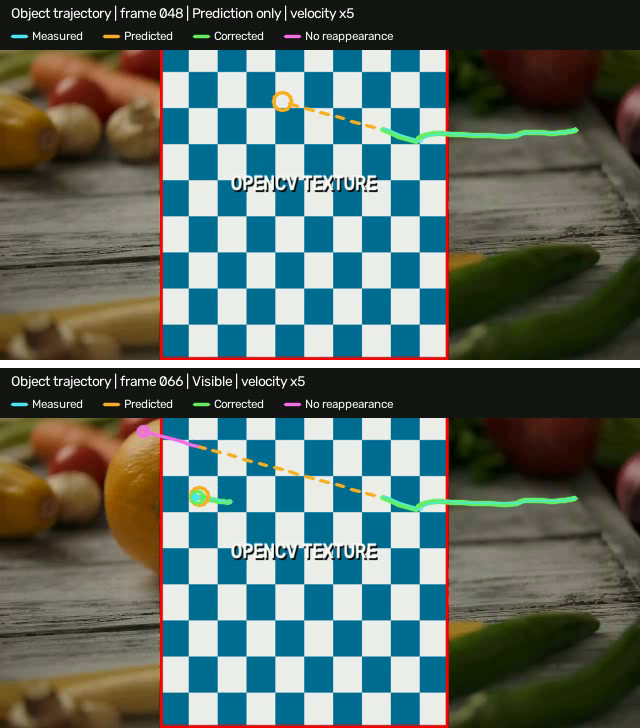
\includegraphics[width=\columnwidth]{clip01-trajectories.png}
\caption{Clip 01 during occlusion (frame 48, top) and after reacquisition
(frame 66, bottom). The orange prediction bridges the gap. The magenta
trajectory continues independently once the live track resumes correction.}
\label{fig:tracks}
\end{figure}

\begin{thebibliography}{2}
\bibitem{lucas1981}
B. D. Lucas and T. Kanade, \textquotedblleft An iterative image registration
technique with an application to stereo vision,\textquotedblright{} in
\emph{Proc. IJCAI}, 1981, pp. 674--678.
\bibitem{kalman1960}
R. E. Kalman, \textquotedblleft A new approach to linear filtering and
prediction problems,\textquotedblright{} \emph{J. Basic Eng.}, vol. 82,
no. 1, pp. 35--45, 1960, doi: 10.1115/1.3662552.
\end{thebibliography}

\end{document}
